\documentclass{standalone}
\usepackage{tikz}
\usetikzlibrary{patterns, positioning}
\usepackage[sfdefault]{ClearSans} %% option 'sfdefault' activates Clear Sans as the default text font
\usepackage[T1]{fontenc}

\begin{document}
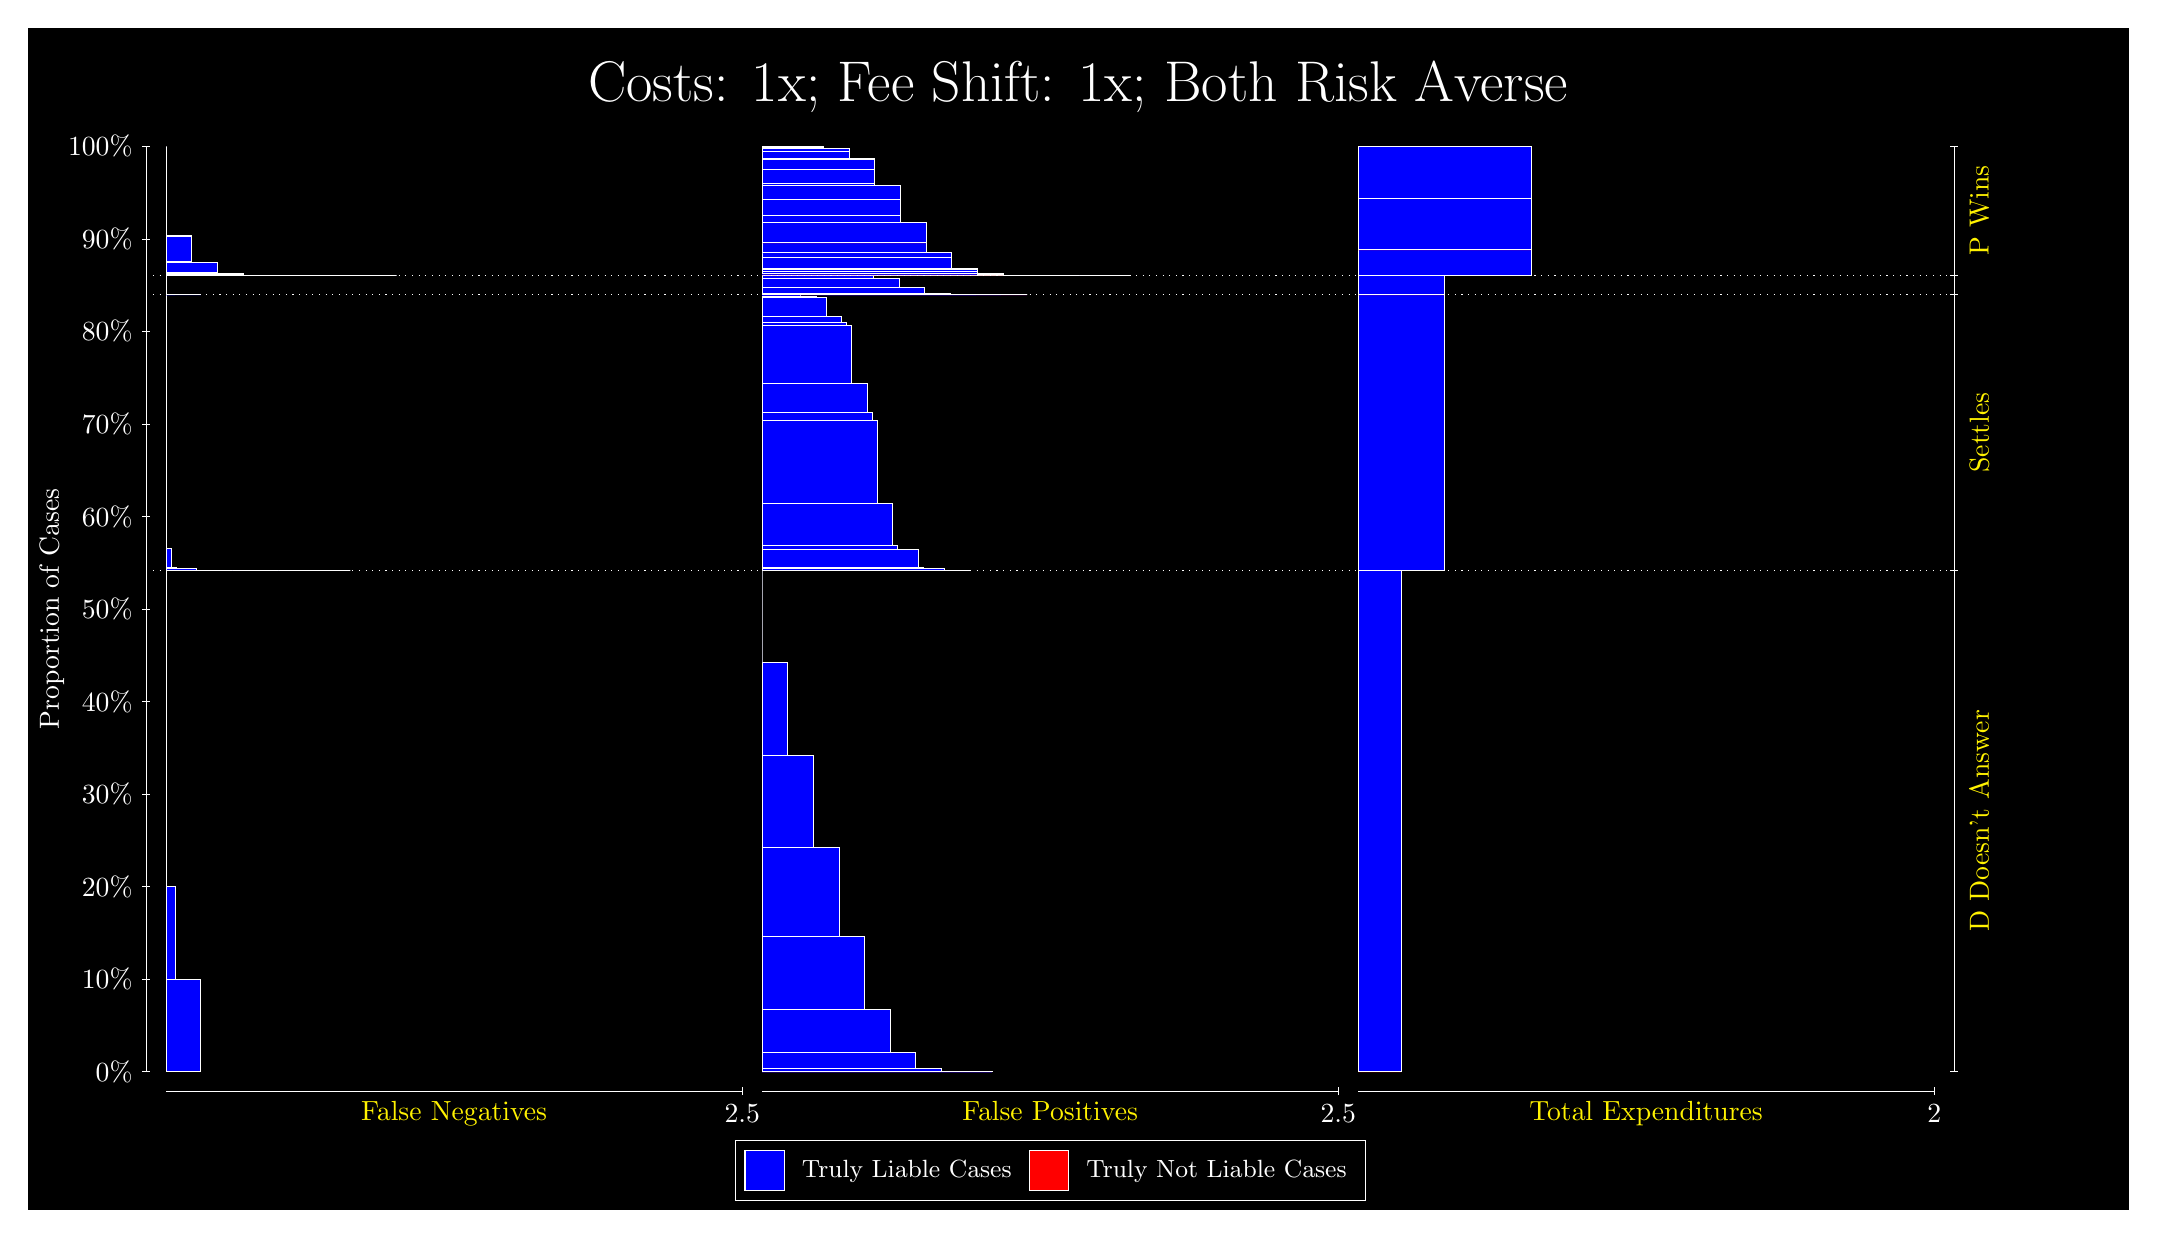
\begin{tikzpicture}
\draw[fill=black] (0,0) rectangle (26.667,15);
\draw[text=white] (0,13.5) rectangle (26.667,15) node[midway] {\huge Costs: 1x; Fee Shift: 1x; Both Risk Averse};
\draw[white, very thin] (1.5,1.75) -- (1.5,13.5);
\node[rotate=90, text=white, anchor=center] at (0.3, 7.625) {Proportion of Cases};
\draw[white, very thin] (1.45,1.75) -- (1.55,1.75);
\node[text=white, anchor=east] at (1.45, 1.75) {0\%};
\draw[white, very thin] (1.45,2.925) -- (1.55,2.925);
\node[text=white, anchor=east] at (1.45, 2.925) {10\%};
\draw[white, very thin] (1.45,4.1) -- (1.55,4.1);
\node[text=white, anchor=east] at (1.45, 4.1) {20\%};
\draw[white, very thin] (1.45,5.275) -- (1.55,5.275);
\node[text=white, anchor=east] at (1.45, 5.275) {30\%};
\draw[white, very thin] (1.45,6.45) -- (1.55,6.45);
\node[text=white, anchor=east] at (1.45, 6.45) {40\%};
\draw[white, very thin] (1.45,7.625) -- (1.55,7.625);
\node[text=white, anchor=east] at (1.45, 7.625) {50\%};
\draw[white, very thin] (1.45,8.8) -- (1.55,8.8);
\node[text=white, anchor=east] at (1.45, 8.8) {60\%};
\draw[white, very thin] (1.45,9.975) -- (1.55,9.975);
\node[text=white, anchor=east] at (1.45, 9.975) {70\%};
\draw[white, very thin] (1.45,11.15) -- (1.55,11.15);
\node[text=white, anchor=east] at (1.45, 11.15) {80\%};
\draw[white, very thin] (1.45,12.325) -- (1.55,12.325);
\node[text=white, anchor=east] at (1.45, 12.325) {90\%};
\draw[white, very thin] (1.45,13.5) -- (1.55,13.5);
\node[text=white, anchor=east] at (1.45, 13.5) {100\%};

\draw[white, very thin] (24.457,1.75) -- (24.457,13.5);
\draw[white, very thin] (24.407,1.75) -- (24.507,1.75);
\node[anchor=west] at (24.407, 1.75) {};
\draw[white, very thin] (24.407,8.1171) -- (24.507,8.1171);
\node[anchor=west] at (24.407, 8.1171) {};
\draw[white, very thin] (24.407,11.617) -- (24.507,11.617);
\node[anchor=west] at (24.407, 11.617) {};
\draw[white, very thin] (24.407,11.865) -- (24.507,11.865);
\node[anchor=west] at (24.407, 11.865) {};
\draw[white, very thin] (24.407,13.5) -- (24.507,13.5);
\node[anchor=west] at (24.407, 13.5) {};

\draw[white, very thin, fill=blue] (1.75,1.75) rectangle (2.1891,2.925);
\draw[white, very thin, fill=blue] (1.75,2.925) rectangle (1.8638,4.0999);
\draw[white, very thin, fill=red] (1.75,4.0999) rectangle (1.75,4.0999);
\draw[white, very thin, fill=blue] (1.75,4.0999) rectangle (1.75,8.1171);
\draw[white, very thin, fill=blue] (1.75,8.1171) rectangle (4.092,8.1171);
\draw[white, very thin, fill=blue] (1.75,8.1171) rectangle (3.7668,8.1171);
\draw[white, very thin, fill=blue] (1.75,8.1171) rectangle (3.5065,8.1171);
\draw[white, very thin, fill=blue] (1.75,8.1171) rectangle (3.4415,8.1171);
\draw[white, very thin, fill=blue] (1.75,8.1171) rectangle (3.1812,8.1171);
\draw[white, very thin, fill=blue] (1.75,8.1171) rectangle (3.1162,8.1171);
\draw[white, very thin, fill=blue] (1.75,8.1171) rectangle (2.921,8.1171);
\draw[white, very thin, fill=blue] (1.75,8.1171) rectangle (2.856,8.1171);
\draw[white, very thin, fill=blue] (1.75,8.1171) rectangle (2.7909,8.1171);
\draw[white, very thin, fill=blue] (1.75,8.1171) rectangle (2.5957,8.1171);
\draw[white, very thin, fill=blue] (1.75,8.1171) rectangle (2.5307,8.1171);
\draw[white, very thin, fill=blue] (1.75,8.1171) rectangle (2.4656,8.1176);
\draw[white, very thin, fill=blue] (1.75,8.1176) rectangle (2.2705,8.1176);
\draw[white, very thin, fill=blue] (1.75,8.1176) rectangle (2.2054,8.1177);
\draw[white, very thin, fill=blue] (1.75,8.1177) rectangle (2.1403,8.1418);
\draw[white, very thin, fill=blue] (1.75,8.1418) rectangle (1.9452,8.1452);
\draw[white, very thin, fill=blue] (1.75,8.1452) rectangle (1.8801,8.1485);
\draw[white, very thin, fill=blue] (1.75,8.1485) rectangle (1.8151,8.395);
\draw[white, very thin, fill=red] (1.75,8.395) rectangle (1.75,8.395);
\draw[white, very thin, fill=blue] (1.75,8.395) rectangle (1.75,11.617);
\draw[white, very thin, fill=blue] (1.75,11.617) rectangle (2.1891,11.617);
\draw[white, very thin, fill=blue] (1.75,11.617) rectangle (1.8638,11.617);
\draw[white, very thin, fill=red] (1.75,11.617) rectangle (1.75,11.617);
\draw[white, very thin, fill=blue] (1.75,11.617) rectangle (1.75,11.865);
\draw[white, very thin, fill=blue] (1.75,11.865) rectangle (4.6775,11.865);
\draw[white, very thin, fill=blue] (1.75,11.865) rectangle (4.3523,11.865);
\draw[white, very thin, fill=blue] (1.75,11.865) rectangle (4.027,11.865);
\draw[white, very thin, fill=blue] (1.75,11.865) rectangle (4.027,11.865);
\draw[white, very thin, fill=blue] (1.75,11.865) rectangle (3.7017,11.865);
\draw[white, very thin, fill=blue] (1.75,11.865) rectangle (3.7017,11.865);
\draw[white, very thin, fill=blue] (1.75,11.865) rectangle (3.3764,11.865);
\draw[white, very thin, fill=blue] (1.75,11.865) rectangle (3.0511,11.865);
\draw[white, very thin, fill=blue] (1.75,11.865) rectangle (3.0511,11.867);
\draw[white, very thin, fill=blue] (1.75,11.867) rectangle (2.7258,11.869);
\draw[white, very thin, fill=blue] (1.75,11.869) rectangle (2.7258,11.89);
\draw[white, very thin, fill=blue] (1.75,11.89) rectangle (2.7258,11.89);
\draw[white, very thin, fill=blue] (1.75,11.89) rectangle (2.4006,11.896);
\draw[white, very thin, fill=blue] (1.75,11.896) rectangle (2.4006,12.022);
\draw[white, very thin, fill=blue] (1.75,12.022) rectangle (2.0753,12.034);
\draw[white, very thin, fill=blue] (1.75,12.034) rectangle (2.0753,12.363);
\draw[white, very thin, fill=blue] (1.75,12.363) rectangle (2.0753,12.364);
\draw[white, very thin, fill=red] (1.75,12.364) rectangle (1.75,12.364);
\draw[white, very thin, fill=blue] (1.75,12.364) rectangle (1.75,13.5);
\draw[white, very thin, fill=red] (9.3189,1.75) rectangle (12.246,1.75);
\draw[white, very thin, fill=blue] (9.3189,1.75) rectangle (12.246,1.7502);
\draw[white, very thin, fill=blue] (9.3189,1.7502) rectangle (11.921,1.7536);
\draw[white, very thin, fill=blue] (9.3189,1.7536) rectangle (11.596,1.7909);
\draw[white, very thin, fill=blue] (9.3189,1.7909) rectangle (11.271,1.9883);
\draw[white, very thin, fill=blue] (9.3189,1.9883) rectangle (10.945,2.5391);
\draw[white, very thin, fill=blue] (9.3189,2.5391) rectangle (10.62,3.4704);
\draw[white, very thin, fill=blue] (9.3189,3.4704) rectangle (10.295,4.5966);
\draw[white, very thin, fill=blue] (9.3189,4.5966) rectangle (9.9694,5.7673);
\draw[white, very thin, fill=blue] (9.3189,5.7673) rectangle (9.6442,6.9421);
\draw[white, very thin, fill=blue] (9.3189,6.9421) rectangle (9.3189,8.1171);
\draw[white, very thin, fill=red] (9.3189,8.1171) rectangle (11.954,8.1171);
\draw[white, very thin, fill=blue] (9.3189,8.1171) rectangle (11.954,8.1181);
\draw[white, very thin, fill=blue] (9.3189,8.1181) rectangle (11.628,8.1448);
\draw[white, very thin, fill=red] (9.3189,8.1448) rectangle (11.368,8.1448);
\draw[white, very thin, fill=blue] (9.3189,8.1448) rectangle (11.368,8.1542);
\draw[white, very thin, fill=blue] (9.3189,8.1542) rectangle (11.303,8.38);
\draw[white, very thin, fill=blue] (9.3189,8.38) rectangle (11.043,8.434);
\draw[white, very thin, fill=blue] (9.3189,8.434) rectangle (10.978,8.9675);
\draw[white, very thin, fill=red] (9.3189,8.9675) rectangle (10.783,8.9675);
\draw[white, very thin, fill=blue] (9.3189,8.9675) rectangle (10.783,10.019);
\draw[white, very thin, fill=blue] (9.3189,10.019) rectangle (10.718,10.119);
\draw[white, very thin, fill=blue] (9.3189,10.119) rectangle (10.653,10.494);
\draw[white, very thin, fill=blue] (9.3189,10.494) rectangle (10.457,11.224);
\draw[white, very thin, fill=blue] (9.3189,11.224) rectangle (10.392,11.265);
\draw[white, very thin, fill=blue] (9.3189,11.265) rectangle (10.327,11.339);
\draw[white, very thin, fill=blue] (9.3189,11.339) rectangle (10.132,11.585);
\draw[white, very thin, fill=blue] (9.3189,11.585) rectangle (10.067,11.589);
\draw[white, very thin, fill=blue] (9.3189,11.589) rectangle (10.002,11.592);
\draw[white, very thin, fill=blue] (9.3189,11.592) rectangle (9.8068,11.616);
\draw[white, very thin, fill=blue] (9.3189,11.616) rectangle (9.7417,11.616);
\draw[white, very thin, fill=blue] (9.3189,11.616) rectangle (9.6767,11.616);
\draw[white, very thin, fill=blue] (9.3189,11.616) rectangle (9.4815,11.617);
\draw[white, very thin, fill=blue] (9.3189,11.617) rectangle (9.4165,11.617);
\draw[white, very thin, fill=blue] (9.3189,11.617) rectangle (9.3514,11.617);
\draw[white, very thin, fill=blue] (9.3189,11.617) rectangle (9.3189,11.617);
\draw[white, very thin, fill=red] (9.3189,11.617) rectangle (12.686,11.617);
\draw[white, very thin, fill=blue] (9.3189,11.617) rectangle (12.686,11.617);
\draw[white, very thin, fill=blue] (9.3189,11.617) rectangle (12.36,11.617);
\draw[white, very thin, fill=blue] (9.3189,11.617) rectangle (12.035,11.617);
\draw[white, very thin, fill=blue] (9.3189,11.617) rectangle (11.71,11.628);
\draw[white, very thin, fill=blue] (9.3189,11.628) rectangle (11.384,11.708);
\draw[white, very thin, fill=blue] (9.3189,11.708) rectangle (11.059,11.822);
\draw[white, very thin, fill=blue] (9.3189,11.822) rectangle (10.734,11.861);
\draw[white, very thin, fill=blue] (9.3189,11.861) rectangle (10.409,11.865);
\draw[white, very thin, fill=blue] (9.3189,11.865) rectangle (10.083,11.865);
\draw[white, very thin, fill=blue] (9.3189,11.865) rectangle (9.758,11.865);
\draw[white, very thin, fill=red] (9.3189,11.865) rectangle (14.003,11.865);
\draw[white, very thin, fill=blue] (9.3189,11.865) rectangle (14.003,11.865);
\draw[white, very thin, fill=red] (9.3189,11.865) rectangle (13.678,11.865);
\draw[white, very thin, fill=blue] (9.3189,11.865) rectangle (13.678,11.865);
\draw[white, very thin, fill=red] (9.3189,11.865) rectangle (13.352,11.865);
\draw[white, very thin, fill=blue] (9.3189,11.865) rectangle (13.352,11.865);
\draw[white, very thin, fill=blue] (9.3189,11.865) rectangle (13.027,11.865);
\draw[white, very thin, fill=red] (9.3189,11.865) rectangle (13.027,11.865);
\draw[white, very thin, fill=blue] (9.3189,11.865) rectangle (13.027,11.865);
\draw[white, very thin, fill=blue] (9.3189,11.865) rectangle (12.702,11.866);
\draw[white, very thin, fill=red] (9.3189,11.866) rectangle (12.702,11.866);
\draw[white, very thin, fill=blue] (9.3189,11.866) rectangle (12.702,11.867);
\draw[white, very thin, fill=blue] (9.3189,11.867) rectangle (12.377,11.872);
\draw[white, very thin, fill=red] (9.3189,11.872) rectangle (12.377,11.872);
\draw[white, very thin, fill=blue] (9.3189,11.872) rectangle (12.377,11.882);
\draw[white, very thin, fill=blue] (9.3189,11.882) rectangle (12.051,11.883);
\draw[white, very thin, fill=red] (9.3189,11.883) rectangle (12.051,11.883);
\draw[white, very thin, fill=blue] (9.3189,11.883) rectangle (12.051,11.912);
\draw[white, very thin, fill=blue] (9.3189,11.912) rectangle (12.051,11.934);
\draw[white, very thin, fill=blue] (9.3189,11.934) rectangle (12.051,11.951);
\draw[white, very thin, fill=blue] (9.3189,11.951) rectangle (11.726,11.952);
\draw[white, very thin, fill=red] (9.3189,11.952) rectangle (11.726,11.952);
\draw[white, very thin, fill=blue] (9.3189,11.952) rectangle (11.726,12.085);
\draw[white, very thin, fill=blue] (9.3189,12.085) rectangle (11.726,12.15);
\draw[white, very thin, fill=blue] (9.3189,12.15) rectangle (11.401,12.15);
\draw[white, very thin, fill=blue] (9.3189,12.15) rectangle (11.401,12.277);
\draw[white, very thin, fill=red] (9.3189,12.277) rectangle (11.401,12.277);
\draw[white, very thin, fill=blue] (9.3189,12.277) rectangle (11.401,12.53);
\draw[white, very thin, fill=blue] (9.3189,12.53) rectangle (11.075,12.627);
\draw[white, very thin, fill=red] (9.3189,12.627) rectangle (11.075,12.627);
\draw[white, very thin, fill=blue] (9.3189,12.627) rectangle (11.075,12.831);
\draw[white, very thin, fill=blue] (9.3189,12.831) rectangle (11.075,13.001);
\draw[white, very thin, fill=blue] (9.3189,13.001) rectangle (10.75,13.035);
\draw[white, very thin, fill=blue] (9.3189,13.035) rectangle (10.75,13.204);
\draw[white, very thin, fill=blue] (9.3189,13.204) rectangle (10.75,13.331);
\draw[white, very thin, fill=blue] (9.3189,13.331) rectangle (10.75,13.343);
\draw[white, very thin, fill=blue] (9.3189,13.343) rectangle (10.425,13.433);
\draw[white, very thin, fill=blue] (9.3189,13.433) rectangle (10.425,13.474);
\draw[white, very thin, fill=blue] (9.3189,13.474) rectangle (10.425,13.475);
\draw[white, very thin, fill=blue] (9.3189,13.475) rectangle (10.1,13.475);
\draw[white, very thin, fill=blue] (9.3189,13.475) rectangle (10.1,13.49);
\draw[white, very thin, fill=blue] (9.3189,13.49) rectangle (10.1,13.498);
\draw[white, very thin, fill=blue] (9.3189,13.498) rectangle (10.1,13.498);
\draw[white, very thin, fill=blue] (9.3189,13.498) rectangle (9.7743,13.499);
\draw[white, very thin, fill=blue] (9.3189,13.499) rectangle (9.7743,13.5);
\draw[white, very thin, fill=blue] (9.3189,13.5) rectangle (9.449,13.5);
\draw[white, very thin, fill=blue] (9.3189,13.5) rectangle (9.449,13.5);
\draw[white, very thin, fill=blue] (9.3189,13.5) rectangle (9.449,13.5);
\draw[white, very thin, fill=blue] (9.3189,13.5) rectangle (9.3189,13.5);
\draw[white, very thin, fill=red] (16.888,1.75) rectangle (17.437,1.75);
\draw[white, very thin, fill=blue] (16.888,1.75) rectangle (17.437,8.1171);
\draw[white, very thin, fill=red] (16.888,8.1171) rectangle (17.986,8.1171);
\draw[white, very thin, fill=blue] (16.888,8.1171) rectangle (17.986,11.617);
\draw[white, very thin, fill=red] (16.888,11.617) rectangle (17.986,11.617);
\draw[white, very thin, fill=blue] (16.888,11.617) rectangle (17.986,11.865);
\draw[white, very thin, fill=red] (16.888,11.865) rectangle (19.083,11.865);
\draw[white, very thin, fill=blue] (16.888,11.865) rectangle (19.083,12.189);
\draw[white, very thin, fill=red] (16.888,12.189) rectangle (19.083,12.189);
\draw[white, very thin, fill=blue] (16.888,12.189) rectangle (19.083,12.841);
\draw[white, very thin, fill=red] (16.888,12.841) rectangle (19.083,12.841);
\draw[white, very thin, fill=blue] (16.888,12.841) rectangle (19.083,13.5);
\draw[white, dotted] (1.5,8.1171) -- (24.457,8.1171);
\draw[white, dotted] (1.5,11.617) -- (24.457,11.617);
\draw[white, dotted] (1.5,11.865) -- (24.457,11.865);
\draw[white, very thin] (1.75,1.5) -- (9.0689,1.5);
\node[text=yellow, anchor=north] at (5.4094, 1.5) {False Negatives};
\draw[white, very thin] (9.0689,1.45) -- (9.0689,1.55);
\node[text=white, anchor=north] at (9.0689, 1.45) {2.5};

\draw[white, very thin] (9.3189,1.5) -- (16.638,1.5);
\node[text=yellow, anchor=north] at (12.978, 1.5) {False Positives};
\draw[white, very thin] (16.638,1.45) -- (16.638,1.55);
\node[text=white, anchor=north] at (16.638, 1.45) {2.5};

\draw[white, very thin] (16.888,1.5) -- (24.207,1.5);
\node[text=yellow, anchor=north] at (20.547, 1.5) {Total Expenditures};
\draw[white, very thin] (24.207,1.45) -- (24.207,1.55);
\node[text=white, anchor=north] at (24.207, 1.45) {2};

\node[text=yellow, centered, rotate=90] at (24.777, 4.9336) {D Doesn't Answer};
\node[text=yellow, centered, rotate=90] at (24.777, 9.867) {Settles};

\node[text=yellow, centered, rotate=90] at (24.777, 12.682) {P Wins};

\draw (12.978300999999998,1.5) node[draw=none] (baseCoordinate) {};
\begin{scope}[align=center]
        \matrix[scale=0.5, draw=white, below=0.5cm of baseCoordinate, nodes={draw}, column sep=0.1cm]{
            \node[rectangle, draw, minimum width=0.5cm, minimum height=0.5cm, fill=blue] {}; &
            \node[draw=none, font=\small, text=white] (B) {Truly Liable Cases}; &
            \node[rectangle, draw, minimum width=0.5cm, minimum height=0.5cm, fill=red] {}; &
            \node[draw=none, font=\small, text=white] (B) {Truly Not Liable Cases}; \\
            };
\end{scope}

\end{tikzpicture}
\end{document}